%!TEX root = ../crimson_throne_book_main.tex
% 2015-02-22
The flesh golem roars as it closes in for the attack. The companions are ready for it, though, having read Rotlh's notes. None of them has an adamantine weapon, so they expect to have trouble getting through its thick hide. They do have a very important advantage, however, fire and ice! Sjo can enhance his strikes with flames and Quint's weapon crackles with frost. Both types of magic are supposed to slow the creature.\\

The companions decide to draw the golem into the entrance cave, where they will be able to surround it. Sjo casts a {\itshape burning hands} on it, while he and his friends get into position. The creature follows in slow motion. Quint also prepares by boosting Balian, Sjo and himself with  {\itshape heroism} and Puk sneaks behind the assailant, sneaking through the shadows. The stitched man finally manages to start hostilities, but his first swing goes high and misses Balian completely. The heroes now encircle the creature and strike from all sides, discovering that its resistance to non-adamantine weapons is not as tough as they expected. Instead of the dreaded encounter to the death, the companions find themselves within the grasp of an easy victory. Sure, the golem manages to score a couple of hits, but since fire of ice keep it slowed, it does not pose much of a threat. A few breaths later it topples to the floor. Quint can't get over how easy this was, considering how complicated and expensive it is to create such a being. The heroes\hyperref[fig:Pathfinder-Foxglove-manor-to-Lost-End-cave-515531738]{ explore the caves further } . The tunnel that smells of sea air leads to a huge cave where docks have been built. One big ship could possibly moor here, although it would be treacherous to navigate the water outside the cliffs. It would definitely take an experienced captain to get a vessel into this cave. Along the walls are some left-over supplies, as well as empty barrels and crates. A small prison to the side holds numerous dead rats. \\

\begin{figure}[h]
	\centering
	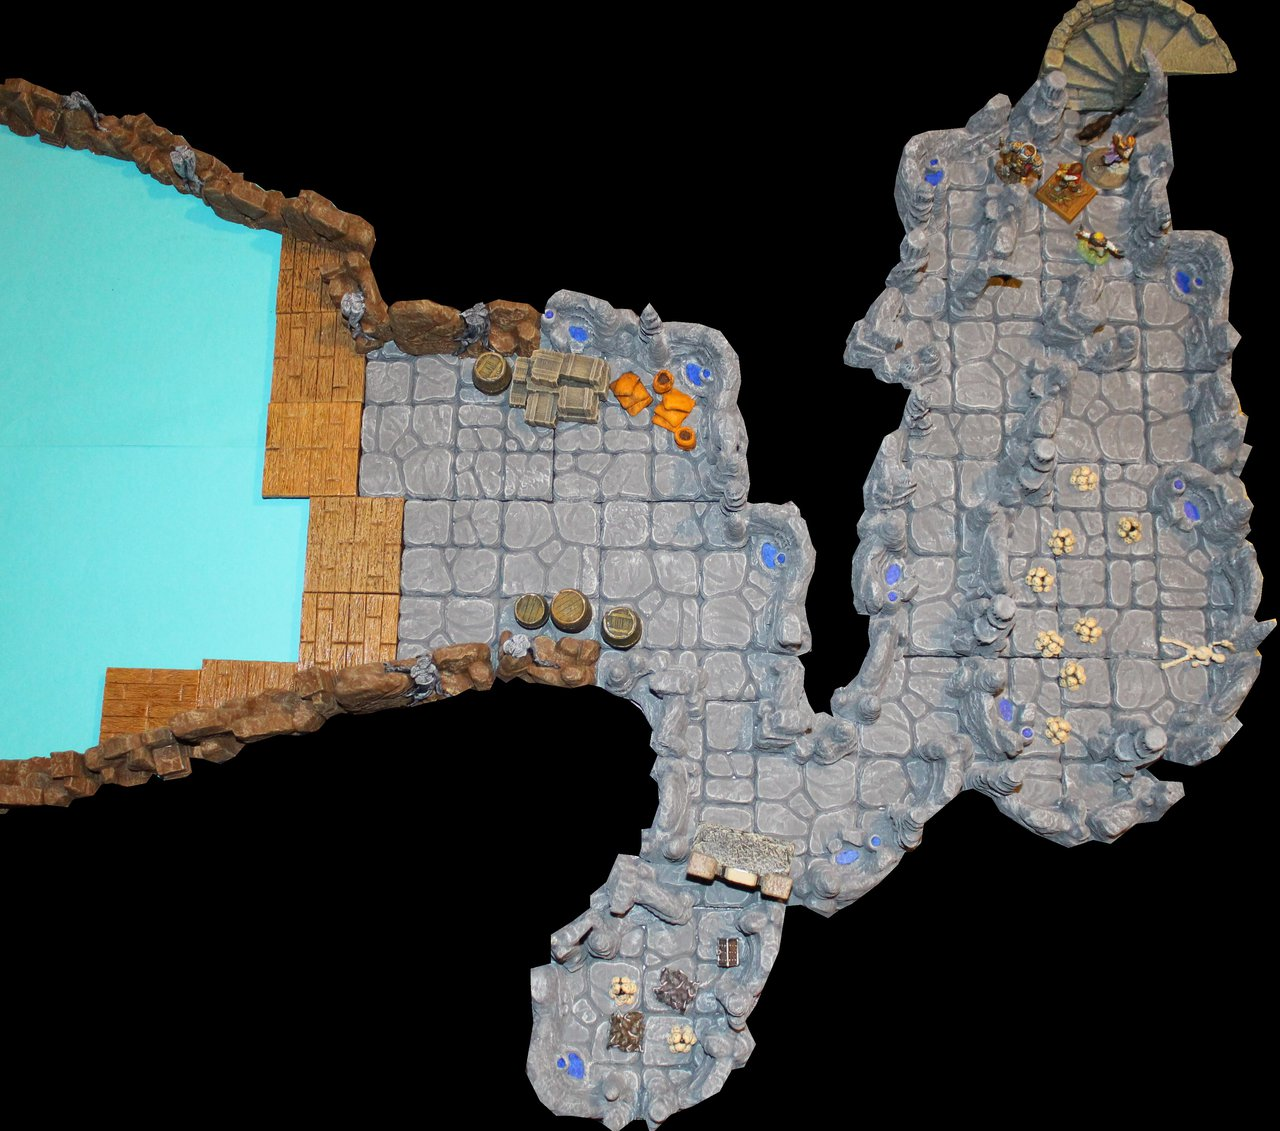
\includegraphics[width=0.39\textwidth]{images/Pathfinder-Foxglove-manor-to-Lost-End-cave-515531738.jpg}
	\caption{Pathfinder Foxglove manor to Lost End cave}
	\label{fig:Pathfinder-Foxglove-manor-to-Lost-End-cave-515531738}
\end{figure}

That leaves only one tunnel, one that reeks of death. With their cloaks in front of their mouths the companions go down the corridor. There is one narrow room at the end that serves as a waste pit filled with hundreds of decaying rodents and a fair number of rotting human corpses. Balian fears that his sister might be one of them, so, despite the overwhelmingly sickening stench, he wants to examine the bodies closer. There turn out to be eleven children here, all girls ... so the lambs that Rolth and the dark-haired lady bought from Gaedran Lamm were sacrificed as guinea pigs! The thought alone leaves the companions foaming at the mouth with anger. Eight corpses are adults, six of which were female as well. Only two had black hair, like Balian's sister, but these two were too old to be Alika. Still, this\hyperref[fig:No-more-mister-Nice-Guy-515533807]{ cruelty will have to be avenged } ! \\

\begin{figure}[h]
	\centering
	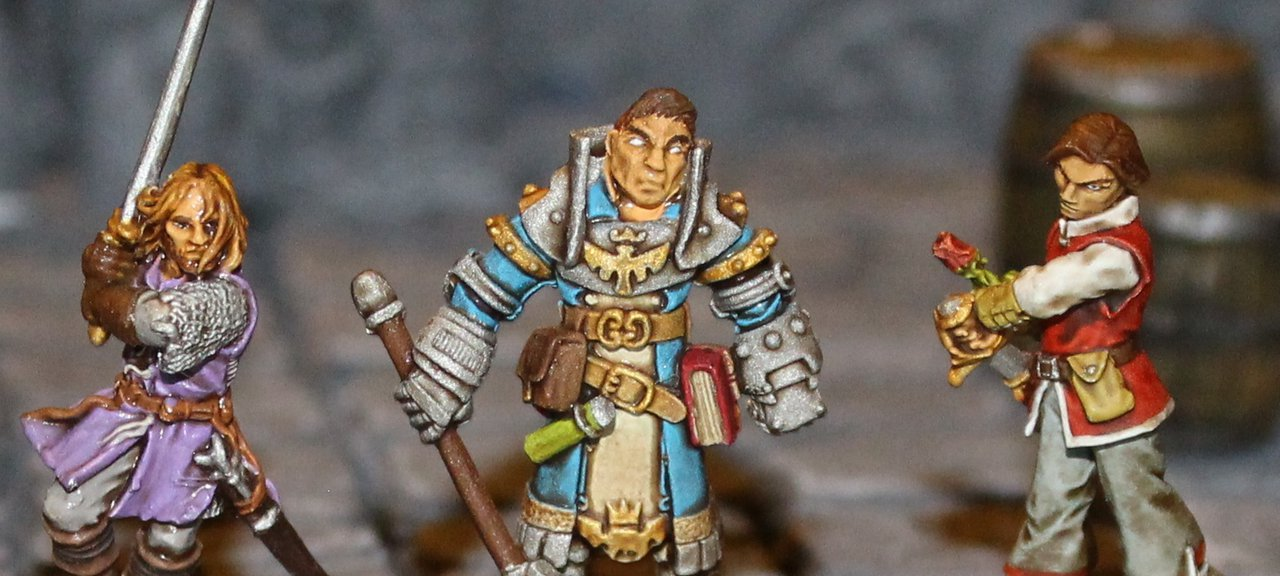
\includegraphics[width=0.39\textwidth]{images/No-more-mister-Nice-Guy-515533807.jpg}
	\caption{No more mister Nice Guy}
	\label{fig:No-more-mister-Nice-Guy-515533807}
\end{figure}

The companions use what is left of the day to make their way back to the Graul hunting lodge, where they spend the night in the barn once again.\\

\section{Level up: level 6!}

\section{5 Erastus 4708}

The companions rise early in the morning and fire their horses on to take them home as fast as possible. They reach the city as the last light slips across the horizon. When they approach Korvosa, they notice two columns of smokes rising from the city: one in the south and another one, more diffused, in the north. Sjo asks a city guard about them. Apparently the number of deaths has increased so much that the Gray District has taken to burning the corpses, explaining the smoke in the south. The fires in the north have another source, though. Since the situation in Old Korvosa has turned so bad, orders have been issued to quarantine the entire district. All the bridges over the Narrows of Saint Alika are being torched, leaving only the one stone bridge, that will be guarded by the Gray Maidens, who will also patrol the shore line to make sure no one sneaks across.\\

The companions decide to look into the situation later tonight. They have been wondering who to trust with the information they gathered in Lost End. Field Marshal Cressida Kroft seems like an obvious choice, but they fear that she will feel obliged to inform the Castle. The queen is still an unclear factor: is she behind this evil or is she an innocent victim? Her behavior at Trinia's trial certainly does not speak to her defense. So that leaves Vencarlo Orisini: the fencing master is definitely on the same side as the companions and his connection to Blackjack, the caped crusader, might prove valuable. Since Vencarlo lives in Old Korvosa, the companions will be able to check out the situation in the north of the city at the same time.\\

First the four young friends head to their villa, to freshen up and have dinner. Madam Nesia and the kids look healthy and they even have a guest: Meep Gildenglare, the old seamstress, is there again. She has taken the liberty of dressing the three boys in smart blue liveries, complete with the pseudodragon symbol and all. Nesia has been doing well, although she admits to sudden bursts of headache from time to time. She still cannot remember anything about her past.\\

After a heartening dinner the companions trek across the city to the stone bridge off Mainshore Boulevard in North Point into Old Korvosa. Upon arriving there, they stumble upon a battlefield. Four score of Gray Maidens have defended the bridge from angry citizens demanding to leave Old Korvosa. At least a hundred of them lie dead on the other bank of the Narrows. It quickly becomes clear that the Queen's guard will not allow anyone across, even if they bear the official seal from Field Marshal Kroft. So informing Vencarlo has suddenly become impossible, unless the heroes try to slip across unnoticed. They decide against it, at least for tonight; too much blood have been spilt already to risk another incident.\\

